% Comment lines start with %
% LaTeX commands start with \

\documentclass[11pt]{article}  % This is an article with font size 11-point;
                               % you can also use 12 point,...

% Packages add features
\usepackage{times}     % font choice
\usepackage{amsmath}   % American Mathematical Association math formatting
\usepackage{amsthm}    % nice formatting of theorems
\usepackage{latexsym}  % provides some more symbols
\usepackage{fullpage}  % uses most of the page (1-inch margins)
\usepackage{verbatim}
\usepackage{graphicx}
\usepackage{subfigure}
\usepackage[colorlinks, linkcolor=blue]{hyperref}

%add algo
\usepackage{algorithm}  
\usepackage{algorithmic} 
\usepackage{graphicx}


\setlength{\parskip}{.1in}  % increase the space between paragraphs

\renewcommand{\baselinestretch}{1.1}  % increase the space between lines

%% you can put more of your own commands, etc. here

% Actual content starts here.
\begin{document}

\begin{center}         % center all the material between begin and end
{\large                % use larger font
CSCE 668, Distributed Algorithms and Systems \\  % \\ is line break
Spring 2019 \\
Project Report \\
Feiyan Yu
}
\end{center}

\begin{comment}
% \bf makes text inside curly braces boldface
{\bf ** Delete the LaTeX hints in your solution. **}


% blank line separates paragraphs.  First line of a paragraph is automatically
% indented.  

\rule{6in}{.1pt}      % horizontal line 6 inches long and .1 point high

\noindent
{\bf LaTeX hints:} 
\begin{itemize}       % makes a bulleted list

\item Math formulas are enclosed in \$ signs, e.g., {\tt \$x + y = z\$}
  becomes $x + y = z$.   % \tt is ``typewriter font''

\item You can make tables using the ``tabular'' environment:

  \begin{center}
  \begin{tabular}{|c|c|}  % two columns, both centered (c), 
                        % divided by vertical lines (|)
  \hline                  % horizontal line
  hello & goodbye         % separate column entries with &
  \\                      % end each line with \\
  \hline
  \hline
  blue & green 
  \\
  \hline
  odd & even 
  \\
  \hline

  \end{tabular}
  \end{center}

\end{itemize}

\rule{6in}{.1pt}       % horizontal line 6 inches long and .1 point high

\end{comment}
%---------------------------------------------------------------------

\noindent
{\bf Introduction}

\rule{6in}{.1pt}       % horizontal line 6 inches long and .1 point high

\noindent
Our project is from the paper "A deterministic distributed algorithm for weighted all pairs shortest paths through pipelining". Shortest path is a popular research field in distributed algorithm. In this paper, the authors presents an algorithm which can calculate the shortest path from different sources. The algorithm solves $(h,k)$-$SSP$ problem, which means that there are $k$ sources which we can arbitrarily assign and every shortest path does not exceed $h$ hop length. If we assign $k$ sources to be all nodes in the graph, then we get APSP( all pairs shortest paths) problem. In an older paper also proposed by the same authors, another algorithm is presented to solve APSP which requires single source shortest path as a sub-routine and introduces the concept of blocker set. The new algorithm therefore can generalize better. This algorithm, like the older version, needs to assume synchronization. The round number needed to complete the $(h,k)$-$SSP$ problem is $2\sqrt{\Delta kh}+k+h$. If we want to solve ASAP and set $k$ to be $n$, then the round number is $2n\sqrt{\Delta} +2n$. All shortest distances are at most $\Delta$. $\Delta$ is a parameter which we need to give to the algorithm. A simple way of getting $\Delta$ is to input the longest path in the graph. The old algorithm will finish in $O(n^\frac{3}{2})$ rounds which is asymptotically worse than $2n\sqrt{\Delta} +2n$.


\noindent
The algorithm runs in CONGEST model in which every link's bandwidth is bounded. Every node only knows its incident edges. The graph can be directed or undirected. The weight of each edge is non-negative. The old algorithm can tolerate negative edges as long as there are no negative cycles. 


%---------------------------------------------------------------------

\noindent
{\bf Algorithm}

\rule{6in}{.1pt}       % horizontal line 6 inches long and .1 point high

An innovative feature of this algorithm is the use of $\kappa$ instead of just weighted distance. More specifically, $\kappa = d*\gamma + l$, where $\gamma = \sqrt{kh/\Delta}$. So $\kappa$ inherits from weighted distance $d$ and hop length $l$. Another interesting part is that every node keeps a list $list_v$ which stores entry $Z$. $Z$ is of the form $[\kappa, d, l, x]$, where $x$ is the source node. Although some path can never be shortest paths, the storage of it can enable the algorithm to terminate in $O(\sqrt{\Delta kh})$. Because there are many variables, it is clearer to see in a table. 


The entries in $list_v$ are sorted in the order $(d,l,x)$. Initially, every node sets their distance to sources infinity. The sources set its distance to itself 0, and add the entry $(0,0,0,v)$ to its own $list_v$. All other non source nodes have an empty $list_v$ at the beginning. $Z.v$ represents the number of entries in $list_v$ for source $x$ which are below and at $Z$. The message sent is in the form $(Z,Z.flag-d^*,Z.v)$. When receiving a message $Z^-$, it first constructs a new entry $Z$ based on that message. The hop length will increment by 1, the distance will add the weight on that edge and $\kappa$ will change accordingly. If the new distance is smaller than the current shortest distance for that source, we then set the shortest distance to the new distance. And if there are less than $Z^-.v$ entries in $list_v$ for source $x$ whose key value $\kappa$ are smaller than $Z.\kappa$, then we just insert that $Z$ to $list_v$. If not, this new $Z$ will never be a shortest path entry and we can just ignore it. 


Because $flag-d^*$ and $p$ are also attached to entry $Z$, in our implementation, we add those two in our $Z$. So now $Z$ is in the form: $(\kappa, d, l, x, flag-d^*, p)$. The graph in presented in a matrix, where -1 means there is no edge between the two nodes and non-negative number shows the weight. 

\begin{table}[h!]
  \begin{center}
    \caption{Global parameters.}
    \begin{tabular}{l|r} % <-- Alignments: 1st column left, 2nd middle and 3rd right, with vertical lines in between
      \hline
      $S$ & set of sources\\
      \hline
      $k$ & number of sources\\
      \hline
      $h$ & maximum number of hops in a shortest path\\
      \hline
      $\Delta$ & maximum weighted distance of a shortest path\\
      \hline
      $n$ & number of nodes\\
      \hline
      $\gamma$ & parameter equal to $\sqrt{kh/\Delta}$\\
    \end{tabular}
  \end{center}
\end{table}

\begin{table}[h!]
  \begin{center}
    \caption{Local variables at node $v$.}
    \begin{tabular}{l|r} % <-- Alignments: 1st column left, 2nd middle and 3rd right, with vertical lines in between
      \hline
      $d^{*}_{x}$ & current shortest path distance from $x$ to $v$\\
      \hline
      $list_v$ & list at $v$ for storing the SP and non-SP entries\\
    \end{tabular}
  \end{center}
\end{table}

\begin{table}[h!]
  \begin{center}
    \caption{Variables for entry $Z=(\kappa,d,l,x)$ in $list_v$.}
    \begin{tabular}{l|r} % <-- Alignments: 1st column left, 2nd middle and 3rd right, with vertical lines in between
      \hline
      $\kappa$ & $\kappa = d*\gamma + l$\\
      \hline
      $d$ & weight (distance) of the path associated with this entry\\
      \hline
      $l$ & hop-length of the path associated with this entry\\
      \hline
      $x$ & start node (i.e. source) of the path associated with this entry\\
      \hline
      $p$ & parent node of $v$ on the path associated with this entry\\
      \hline
      $v$ & number of entries for source $x$ at or below $Z$ in $list_v$ (not stored explicitly)\\
      \hline
      $flag-d^*$ & flag to indicate if $Z$ is the current SP entry for source $x$\\
      \hline
      $pos$ & position of $Z$ in $list_v$ in a round r
    \end{tabular}
  \end{center}
\end{table}

\begin{algorithm}[!h]
    \caption{$(h,k)-SSP$ algorithm}%    算法r标题
    \hspace*{0.02in} Initialization for node $v$:
    \begin{algorithmic}[1]
        \STATE for each $x \in S$ do $d^{*}_{x} \gets \infty$
        \STATE if $v \in S$ then $d^{*}_{x} \gets 0$; add entry $Z=(0,0,0,v)$ to $list_v$; $Z.flag-d^* \gets true$
    \end{algorithmic}
    
    \hspace*{0.02in} Algorithm at node $v$ for round $r$:
    \begin{algorithmic}[1]
        \STATE send: if there is an entry $Z$ with $\lceil Z.\kappa + pos(Z) = r \rceil $
        \STATE ~~~~then compute $Z.v$ and form the message $M = <Z, Z.flag-d^*, Z.v>$ and send $M$ to all neighbors.
        
        \STATE receive: let $I$ be the set of incoming messages
        \STATE for each $M \in I$ do 
        \STATE ~~~~let $M = (Z^- = (\kappa ^-, d^-, l^-,x), Z^-.flag-d^*, Z^-.v) $ and let the sender be $y$
        \STATE ~~~~$\kappa \gets \kappa ^- + w(y,v)*\gamma + 1$; $d \gets d^- +w(y,v)$; $l \gets l^- +1$
        \STATE ~~~~$Z \gets (\kappa, d, l, x)$; $Z.flag-d^* \gets false$; $Z.p \gets y$
        \STATE ~~~~let $Z^*$ be the entry for $x$ in $list_v$ such that $Z^*.flag-d^* = true$ if such an entry exists.
        \STATE ~~~~if $Z^-.flag-d^*=true$ and $l<=h$ and ($(d<d^{*}_{x})$ or $(d=d^{*}_{x}$ and $Z.l< Z^*.l)$ or $(d=d^{*}_{x}$ and $Z.l = Z^*.l$ and $Z.p < Z^*.p)$ 
        \STATE ~~~~then $d^{*}_{x} \gets d$; $Z.flag-d^* \gets true$
        \STATE ~~~~~~~~if $Z^*$ exists
        \STATE ~~~~~~~~~~~~$Z^-.flag-d^*=false$
        \STATE ~~~~~~~~INSERT($Z$)
        \STATE ~~~~else
        \STATE ~~~~~~~~if there are less than $Z^-.v$ entries for $x$ with $key \leq Z.\kappa$ then INSERT($Z$)
    \end{algorithmic}
    
    \hspace*{0.02in} INSERT(Z):
    \begin{algorithmic}[1]
        \STATE insert $Z$ in $list_v$ in sorted order of $(\kappa,d,x)$
        \STATE if $\exists$ an entry $Z'$ for $x$ in $list_v$ such that $Z'.flag-d^* = false$ and $pos(Z')>pos(Z)$ then 
        \STATE ~~~~find $Z'$ with smallest $pos(Z')$ such that $pos(Z')>pos(Z)$ and $Z'.flag-d^* = false$ 
        \STATE ~~~~remove $Z'$ from $list_v$
    \end{algorithmic}
    
\end{algorithm}

% \begin{figure}[h!]
% \centering
% \includegraphics[width=1.0\textwidth]{EX8_9.png}
% \caption{Exercise 8.9}
% \end{figure}

\newpage
\noindent
{\bf Implementation}

\rule{6in}{.1pt}       % horizontal line 6 inches long and .1 point high

\begin{enumerate}
    \item Implementation of Graph API
    
    This algorithm is based on graph, so we built a graph class with some APIs for implementing the main algorithm.
    We used adjacency matrix to show the weights in the graph. What we need is to find the neighbors for each vertex and get the weight of each edge.
    
    \item Simulation of global round number in synchronous case
    
    As for the tool in this project, DistAlgo, has a nature of asynchronous condition. So, it could not resolve the synchronous case directly, also, users could not add a global variables directly for each process. However, the requirement of this algorithm needs every process to know the round number even if this process does not receive any message in this round. So, after each round of sending message of shortest path, we implemented a synchronization step for making sure all the processes could successfully get into the same round. 
    
    Our strategy was simple at this step. We made all the processes send messages to every process contains the local round number. After receiving all the messages with the same round number as the local, the local round number increment by 1. 
    
    \begin{algorithm}[htb] 
    \caption{Round Number Synchronization for process $p_i$} 
    \label{alg:Framwork} 
    \begin{algorithmic}[1] %这个1 表示每一行都显示数字
    \REQUIRE ~~\\ %算法的输入参数:Input
    Initially $p_i.round = 0$ and $p_i.received\_count = 0$ \\
    First Send message:\\
    \STATE send message $M = <p_i.round>$ to the all $n$ processes(including itself) and wait for receiving messages
    
    Then Receive message M:\\
    \IF{$M.round == p_i.round$}
    \STATE $p_i.received\_count = p_i.received\_count + 1$
    \ELSE
    \STATE put M into buffer for later review
    \ENDIF
    \IF{$p_i.received\_count == n$}
    \STATE $p_i.round = p_i.round + 1$
    \STATE Terminate
    \ENDIF
    \end{algorithmic}
    \end{algorithm}
    
    \begin{itemize}
        \item[Termination:] Without any failures, all message should be received. So, before terminate, the process should receive n messages. If all the n message has the same round number, the algorithm terminate.
        \item[Correctness:]Without any failures, this synchronization could ensure that all the processes terminates, all process are at the same round.
        \item[Proof:] 
        
        Lemma 1: At any stage, $p_i.round - p_j.round \leq 1$.
        Proof: If $p_i.round - p_j.round > 1$, that means $p_i$ have received n message $M.round = p_i.round - 1 > o_j.round$. Because there is no duplicated message and no failure, the n message must include a message with round number $M.round = p_i.round - 1$ send by $p_j$. It raises contradiction because $p_j$ could not send a message with round number greater than its round.  
        
        So, the after the slowest processor terminates, and has not send the synchronization message at the next round, all the processes have the same round number. Because during the period between the slowest process terminates and it send the synchronization message for the next round, all processors has the same round number, we could use that time to implement our algorithm. Even if the actual situation is asynchronous, all the process uses the same and correct round number as a parameter. We could think that round number is global now. 
    \end{itemize}
    
    \rule{6in}{.1pt}       % horizontal line 6 inches long and .1 point high
    
    \item Implementation of (h,k)-SSP algorithm
    
    The implementation of the algorithm strictly followed the steps of the (h,k)-SSP in the paper. Because the round number only serve as the condition to determine whether $p_i$ should send message or not, we just user the time interval when all process has the same round number to check it and send (h,k)-SSP message.
    
    The overall step of this implementation is showed below:
        \begin{algorithm}[htb] 
        \caption{(h,k)-SSP(hop, $r_{limits}$, $\Delta$, Graph, Sources)} 
        \label{alg:Framwork} 
        \begin{algorithmic}[1] %这个1 表示每一行都显示数字
        \REQUIRE ~~\\ %算法的输入参数:Input
        \STATE Initialization of loacal variable.
        \WHILE{$p_i.round < r_{limit}$}
        \STATE ASPS\_algorithm()
        \STATE Synchronization()
        \ENDWHILE
        \end{algorithmic}
        \end{algorithm}
   
    
\end{enumerate}

{\bf Results}

\rule{6in}{.1pt}       % horizontal line 6 inches long and .1 point high

We test our algorithm on different graphs, and compare the result with another APSP algorithm - Dijkstra's algorithm. As for the comparison, we use some example at \href{https://visualgo.net/en/sssp}{Visualgo} .\par

The first example is a weighted directed acyclic graphs, and the topology of the graph is as figure 1.

\begin{figure}[ht]
\centering
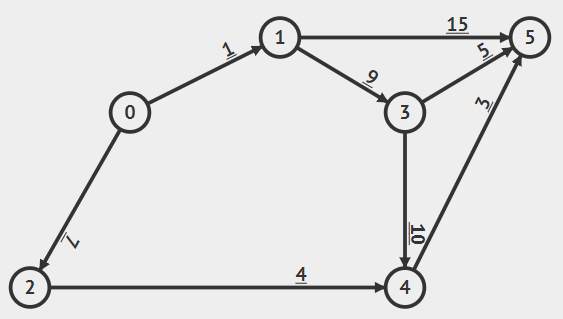
\includegraphics[width=9cm]{dag/0.png}
\caption{Test graph 1}
\end{figure}\par

The following is the mapping between processor's name and the node id.\par

\begin{equation}\nonumber
\begin{aligned}
<P:bfc04>&: 0, 
<P:bfc02>&: 1, \\
<P:bfc07>&: 2, 
<P:bfc03>&: 3, \\
<P:bfc05>&: 4, 
<P:bfc06>&: 5. \\
\end{aligned}
\end{equation}\par
Then the following table shows the results of our algorithm.\par 

\begin{table}[!htbp]
\centering
\setlength{\tabcolsep}{1mm}
\begin{tabular}{|c|c|c|c|c|c|c|}
\hline
processor&$\langle P:bfc04 \rangle$&$\langle P:bfc02\rangle$&$\langle P:bfc07\rangle$&$\langle P:bfc03\rangle$&$\langle P:bfc05\rangle$&$\langle P:bfc06\rangle$\\
\hline
$\langle P:bfc04\rangle$&0&$inf$&$inf$&$inf$&$inf$&$inf$\\
\hline
$\langle P:bfc02\rangle$&1&0&$inf$&$inf$&$inf$&$inf$\\
\hline
$\langle P:bfc07\rangle$&7&$inf$&0&$inf$&$inf$&$inf$\\
\hline
$\langle P:bfc03\rangle$&10&9&$inf$&0&$inf$&$inf$\\
\hline
$\langle P:bfc05\rangle$&11&19&4&10&0&$inf$\\
\hline
$\langle P:bfc06\rangle$&14&14&7&5&3&0\\
\hline
\end{tabular}
\caption{Result of our algorithm on graph 2}
\end{table}\par

Then we compare the result of shortest path of single sources (corresponding to each column in the table) from \href{https://visualgo.net/en/sssp}{Visualgo}'s Dijkstra's algorithm.\par

\begin{figure}[htbp]
\centering
\subfigure[source: node 0]{
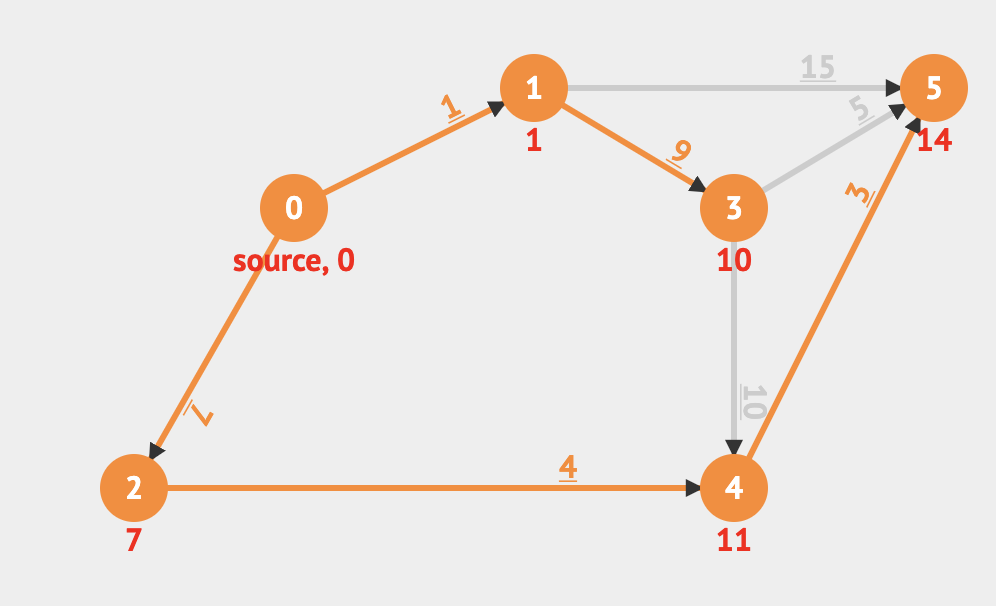
\includegraphics[width=5cm]{dag/source0.png}
}
\quad
\subfigure[source: node 1]{
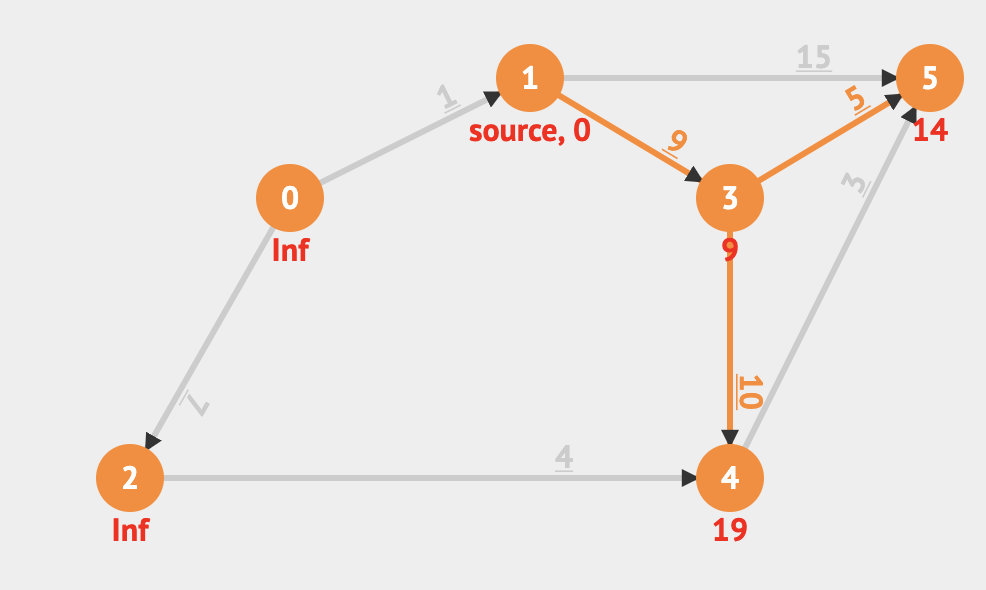
\includegraphics[width=5cm]{dag/source1.png}
}
\quad
\subfigure[source: node 2]{
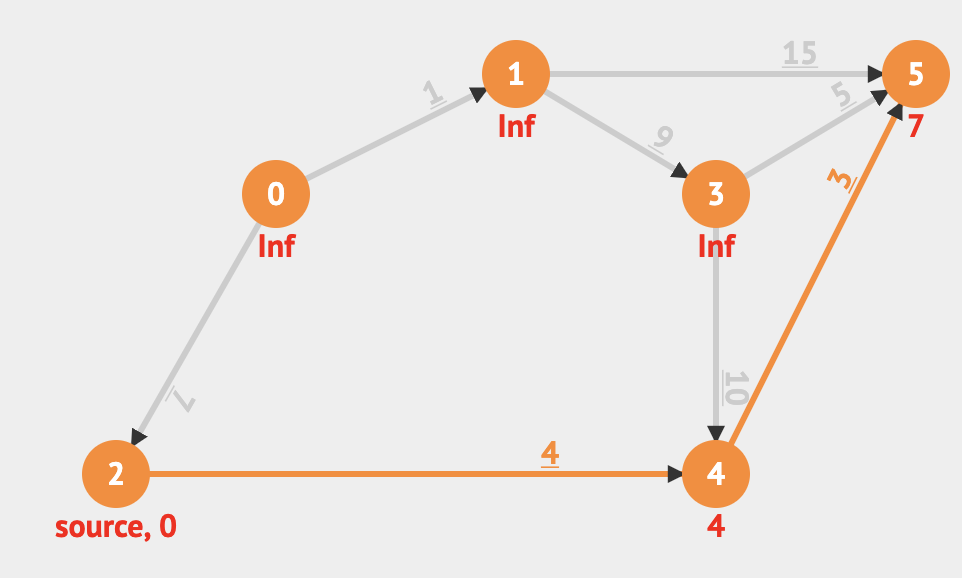
\includegraphics[width=5cm]{dag/source2.png}
}
\quad
\subfigure[source: node 3]{
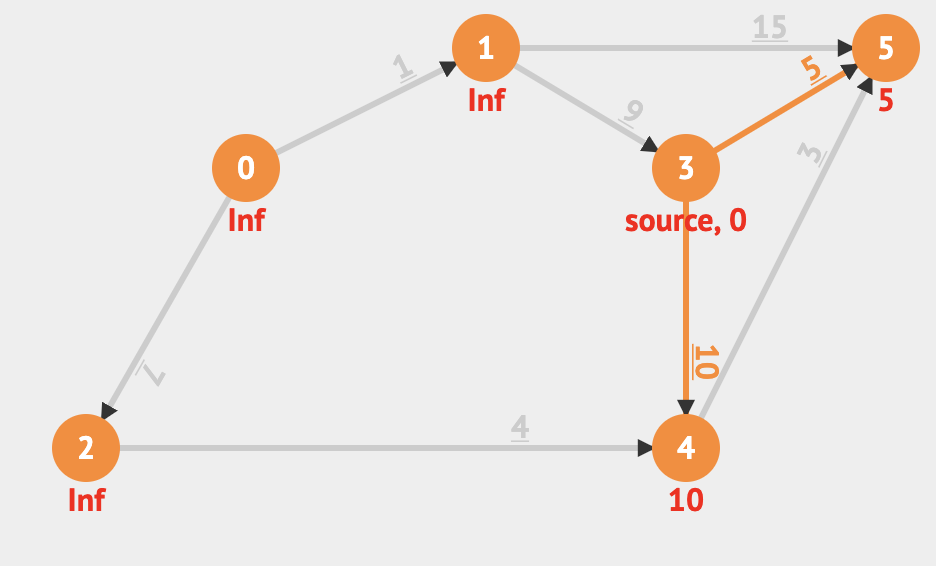
\includegraphics[width=5cm]{dag/source3.png}
}
\quad
\subfigure[source: node 4]{
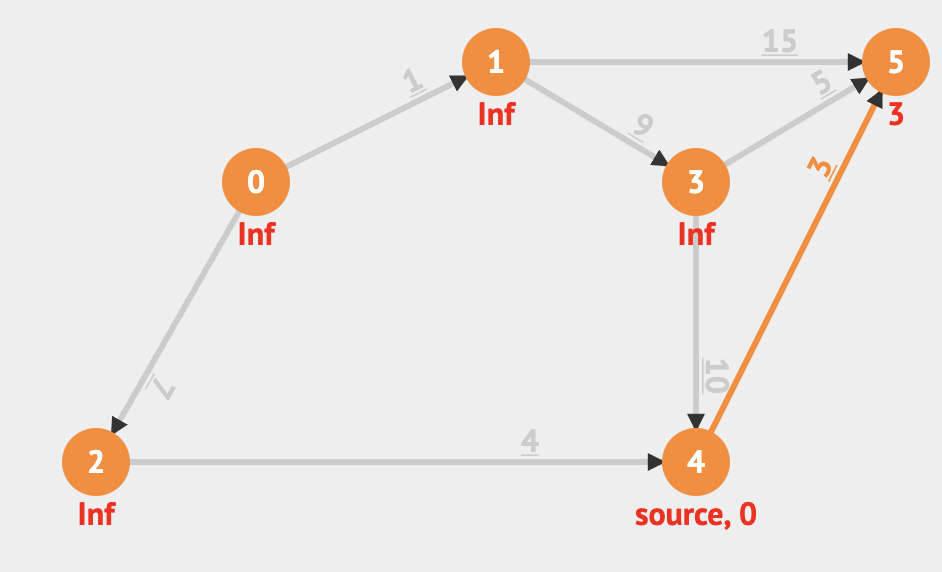
\includegraphics[width=5cm]{dag/source4.png}
}
\quad
\subfigure[source: node 5]{
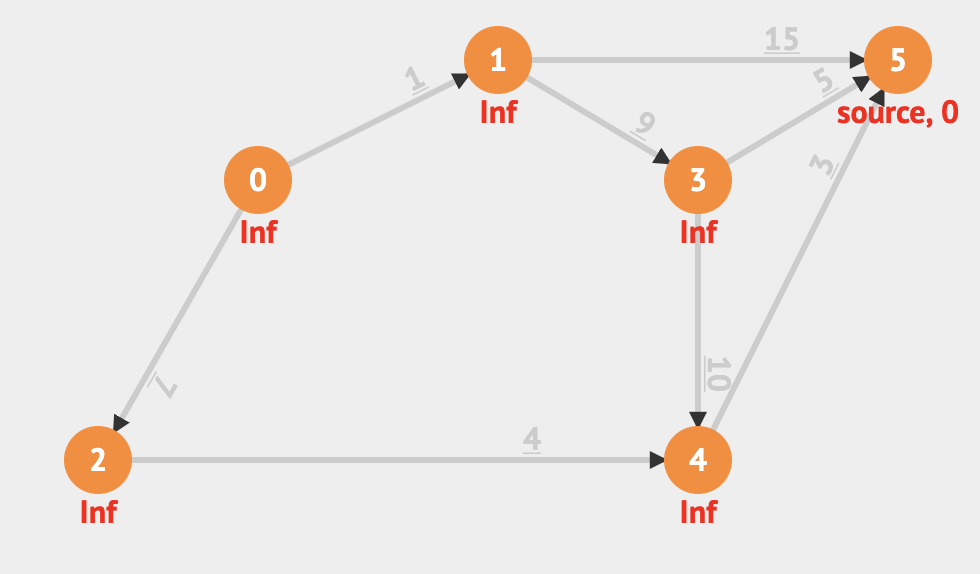
\includegraphics[width=5cm]{dag/source5.png}
}
\caption{ Result of graph 1 from visualgo}
\end{figure}

The second example is a weighted undirected tree, and the topology of the graph is as figure 3.

\begin{figure}[ht]
\centering
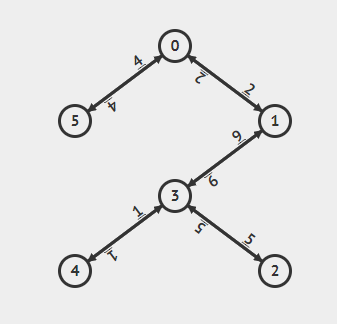
\includegraphics[width=4cm]{CP3_440Tree/CP3_440.png}
\caption{Test graph 2}
\end{figure}\par

The following is the mapping between processor's name and the node id.\par

\begin{equation}\nonumber
\begin{aligned}
<P:47003>&: 0, 
<P:47007>&: 1, \\
<P:47004>&: 2, 
<P:47002>&: 3, \\
<P:47005>&: 4, 
<P:47006>&: 5. \\
\end{aligned}
\end{equation}\par
Then the following table shows the results.\par 

\begin{table}[!htbp]
\centering
\setlength{\tabcolsep}{1mm}
\begin{tabular}{|c|c|c|c|c|c|c|}
\hline
processor&$\langle P:bfc04 \rangle$&$\langle P:bfc02\rangle$&$\langle P:bfc07\rangle$&$\langle P:bfc03\rangle$&$\langle P:bfc05\rangle$&$\langle P:bfc06\rangle$\\
\hline
$\langle P:bfc04\rangle$&0&2&13&8&9&4\\
\hline
$\langle P:bfc02\rangle$&2&0&11&6&7&6\\
\hline
$\langle P:bfc07\rangle$&13&11&0&5&6&$inf$\\
\hline
$\langle P:bfc03\rangle$&8&6&5&0&1&12\\
\hline
$\langle P:bfc05\rangle$&9&7&6&1&0&$inf$\\
\hline
$\langle P:bfc06\rangle$&4&6&$inf$&12&13&0\\
\hline
\end{tabular}
\caption{Result of our algorithm on graph 3}
\end{table}\par

Then the result of shortest path of single sources (corresponding to each column in the table) from \href{https://visualgo.net/en/sssp}{Visualgo}'s Dijkstra's algorithm.\par

\begin{figure}[htbp]
\centering
\subfigure[source: node 0]{
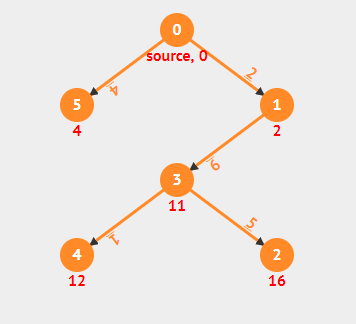
\includegraphics[width=4cm]{CP3_440Tree/CP3_440Tree0start.png}
}
\quad
\subfigure[source: node 1]{
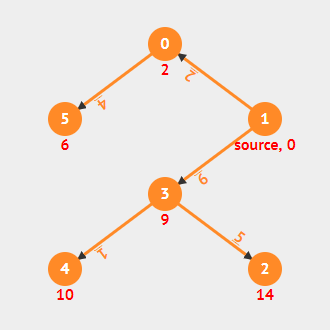
\includegraphics[width=4cm]{CP3_440Tree/CP3_440Tree1start.png}
}
\quad
\subfigure[source: node 2]{
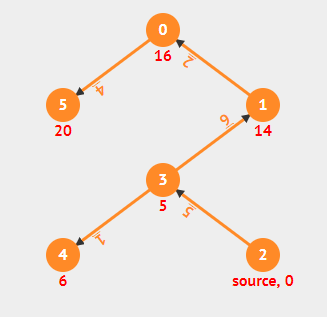
\includegraphics[width=4cm]{CP3_440Tree/CP3_440Tree2start.png}
}
\quad
\subfigure[source: node 3]{
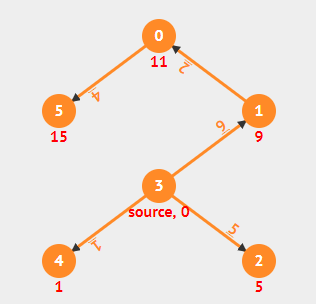
\includegraphics[width=4cm]{CP3_440Tree/CP3_440Tree3start.png}
}
\quad
\subfigure[source: node 4]{
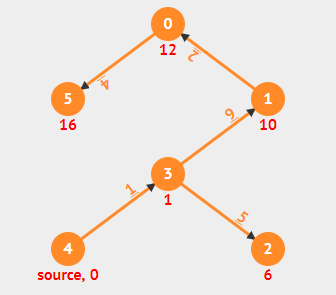
\includegraphics[width=4cm]{CP3_440Tree/CP3_440Tree4start.png}
}
\quad
\subfigure[source: node 5]{
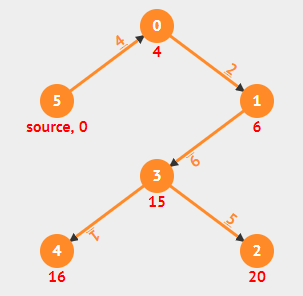
\includegraphics[width=4cm]{CP3_440Tree/CP3_440Tree5start.png}
}
\caption{ Result of graph 2 from visualgo}
\end{figure}\par

The following three example are two negative weighted examples and a graph with a zero weight edge.\par

In the graph with a zero weight edge, the algorithm will give the shortest path without including the zero weight unless the zero weight edge is necessary for the path. In result we also give the parent of node on the shortest path.\par

\begin{figure}[htbp]
\centering
\subfigure[original graph]{
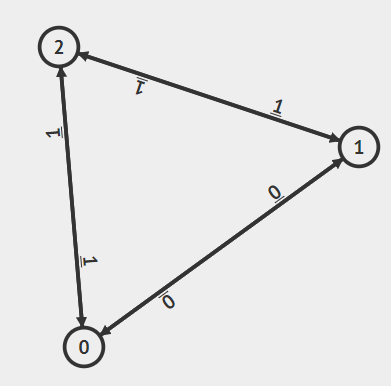
\includegraphics[width=4cm]{zero_weight/-1.png}
}
\quad
\subfigure[source: node 2]{
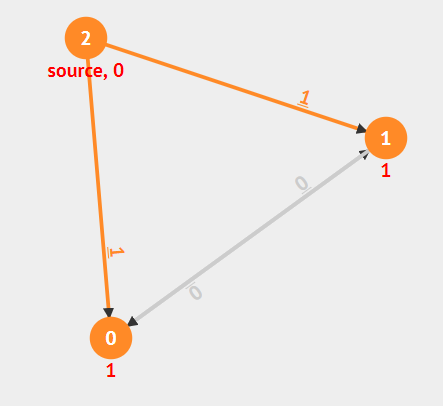
\includegraphics[width=4cm]{zero_weight/2.png}
}
\caption{ graph with a zero weight edge}
\end{figure}\par

The following is output of the algorithm. As for source node 2, both node 0 and node one's immediate parent is node 2, which means since the zero weight edge is not necessary for the shortest path, it is not included.\par
\noindent
\rule{3in}{.1pt}
\noindent \\
source $\langle P:81004\rangle$:2\\
$\langle P:81002\rangle$: 0's parent =  $\langle P:81004\rangle$\\
$\langle P:81003\rangle$: 1's parent =  $\langle P:81004\rangle$\\
output = {$\langle P:81004\rangle$: 1}\\
output = {$\langle P:81004\rangle$: 1}\\
output = {$\langle P:81004\rangle$: 0}\\
\rule{3in}{.1pt}\par

In graph with negative weight edges, the algorithm is not able to give the correct answer. \par

\begin{figure}[htbp]
\centering
\subfigure[graph with only one negative edge]{
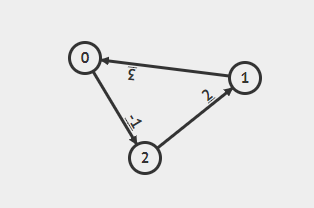
\includegraphics[width=4cm]{negativeEdge/negativeEdge.png}
}
\quad
\subfigure[graph with negative cycle]{
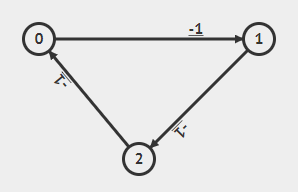
\includegraphics[width=4cm]{negativeCycle/negativeCycle.png}
}
\caption{ Two counter examples}
\end{figure}\par

Judging from the output of the algorithm and comparing with the correct result, the algorithm gives the wrong result.\par

\begin{figure}[htbp]
\centering
\subfigure[source: node 0]{
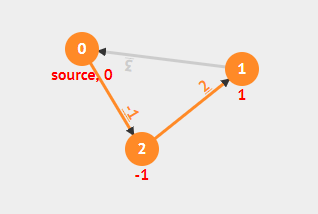
\includegraphics[width=4cm]{negativeEdge/negativeEdge0start.png}
}
\quad
\subfigure[source: node 1]{
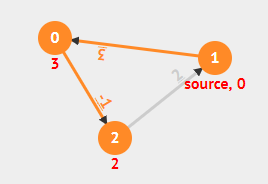
\includegraphics[width=4cm]{negativeEdge/negativeEdge1start.png}
}
\quad
\subfigure[source: node 2]{
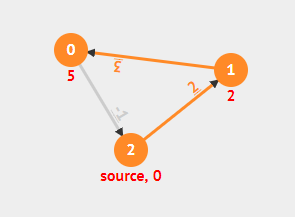
\includegraphics[width=4cm]{negativeEdge/negativeEdge2start.png}
}
\caption{ Visualgo result for the first counter example}
\end{figure}\par

\noindent
\rule{5in}{.1pt}
\noindent \\
{$\langle P:11002\rangle $: 0, $\langle P:11003\rangle$: 1,$\langle P:11004\rangle$: 2}\\
$\langle P:11002\rangle$:OUTPUT: output = {$\langle P:11002\rangle$: 0, $\langle P:11003\rangle$: 3, $\langle P:11004\rangle$: 5}\\
$\langle P:11003\rangle$:OUTPUT: output = {$\langle P:11002\rangle$: $inf$, $\langle P:11003\rangle$: 0, $\langle P:11004\rangle$: 2}\\
$\langle P:11004\rangle$:OUTPUT: output = {$\langle P:11002\rangle$: -1, $\langle P:11003\rangle$: 2, $\langle P:11004\rangle$: 0}\\
\rule{5in}{.1pt}\par

It is known that there is no answer to the shortest path on negative weight cycle, but some algorithms like Bellman Ford's algorithm could detect negative cycle in the graph. After testing the negative weight cycle on this algorithm, it gives the same answer no matter how many rounds or hops we set. The answer is following.\par

\noindent
\rule{5in}{.1pt}
\noindent \\
{$\langle P:4c002\rangle $: 0, $\langle P:4c003\rangle$: 1,$\langle P:4c004\rangle$: 2}\\
$\langle P:4c002\rangle$:OUTPUT: output = {$\langle P:4c002\rangle$: 0, $\langle P:4c003\rangle$: $inf$, $\langle P:4c004\rangle$: -1}\\
$\langle P:4c003\rangle$:OUTPUT: output = {$\langle P:4c002\rangle$: -1, $\langle P:4c003\rangle$: 0, $\langle P:4c004\rangle$: $inf$}\\
$\langle P:4c004\rangle$:OUTPUT: output = {$\langle P:4c002\rangle$: $inf$, $\langle P:4c003\rangle$: -1, $\langle P:4c004\rangle$: 0}\\
\rule{5in}{.1pt}\par


{\bf Conclusion}

\rule{6in}{.1pt}       % horizontal line 6 inches long and .1 point high

This algorithm is a strong and simple algorithm for finding shortest paths for $k$ sources. The round for all pairs shortest paths when $k$ is set to $n$ is $2n\sqrt{\Delta} +2n$, which is linear to $n$. Although every node has to keep a list $list_v$ locally, the number of entries in the list is at most $\sqrt{\Delta h/k}+1$, which is acceptable. 

We use DistAlgo to implement this algorithm and the results are correct. This algorithm avoids going through edges with big weights because at every round, an entry $Z=(\kappa, d, l, x)$ would be sent only when $\lceil Z.\kappa + pos(Z) = r \rceil $, so if the edge weight is too big, $\kappa$ would also be very big, then this entry will be sent at a very late round. This strategy helps early termination and avoids sending useless message. But this strategy makes the algorithm not usable to negative edges. When a negative edge is present, then $\kappa$ can be negative. When the algorithm is checking whether $\lceil Z.\kappa + pos(Z) = r \rceil $, this equation can never be satisfied because this entry is less than round number $r$ and $r$ is always increasing.

\end{document}
